\section{Baseline Results for Synthetic and Real Data}
\label{sec:evaluation}

Later in this work, the effects of pose normalization in the system by \citet{drover18} will be analyzed, both theoretically and experimentally.
In a first step towards the experimental analysis, baseline results for a re-implemented version of the system have to be established.
Those results provide insights about the system's performance under different circumstances and ease a comparison between the original system by \citet{drover18} and modified versions of this system, which will be presented in later sections.

\subsection{Training Procedure and Hyperparameters}
For training, the Adam Optimizer \cite{kingma17} with an initial learning rate of $2 \cdot 10^{-4}$ and $\beta_1 = 0.5$ is used for both generator and discriminator.
This particular choice of $\beta_1$ has shown to result in faster convergence.
As in the work by \citet{drover18}, the data is split up into batches of $32768$ poses.
Generator and discriminator are trained alternately with the same batch of poses, for up to $50000$ iterations until convergence.
Before adjusting the networks' parameters, adaptive clipping is applied to the gradients \cite[Section~3.2.1]{chorowski14}.


\subsection{Results for Training with Synthetic Data}
\label{sec:results-synthetic}

The 2D input poses of the system are required to fulfill the constraints (A) and (B) from \autoref{sec:network-architecture}. 
They state that the poses' root joint has to be centered at the origin of the image plane and that the poses are required to have a norm limb length of $0.1$, that is, be normalized in location and scale.
For an input pose to match those constraints there are two options:
\begin{enumerate}
	\item The input pose already naturally fulfills the constraints by being projected with certain extrinsic camera parameters.
	\item The input pose does not fulfill the constraints and has to be transformed using translation and scaling.
\end{enumerate}
In order to analyze the effects of the normalization in the second case, poses that do not fulfill the constraints are compared to poses that already naturally satisfy them.
Thus, a baseline for (1) has to be established.
For this, the 2D poses included in the Human3.6M are not viable because the cameras used to project the 3D poses do not have the special extrinsic parameters required.
Informally, those parameters can be described as follows:
The camera has to be centered at the root joint (in order to fulfill (A)) and the camera distance to the 3D pose has to be such that the projected norm limb has a length of 0.1 (in order to fulfill constraint (B)).

To obtain suitable poses, synthetic 2D poses are generated by projecting the 3D poses included in Human3.6M with those extrinsic parameters.
For training and testing, cameras centered at the root joint with integer azimuth and elevation angles randomly sampled from $[0, 359]$ degrees and $[0, 20]$ degrees are used.
This choice of elevation angles is based on the same heuristic as in \autoref{sec:network-architecture} and also on the fact that the cameras in Human3.6M have similar angles.
For projection, the 3D poses are first normalized such that the norm limb has length $1$ and then projected with a camera-root-joint distance of $10$ units and a focal length of $1$.
With the specific choice of elevation angles, the projected root limb has a length usually close to 0.1 and only slight scaling is necessary.
For training, \citet{drover18} follow a similar procedure and augment synthetic 2D poses, although they use 8 fixed cameras instead of randomly sampled camera angles for each pose.

\begin{table}[]	
	\centering
	\begin{tabularx}{\textwidth}{l *{8}{Y}}
		\toprule
		Method & Direct. & Discuss & Eat & Greet & Phone & Pose & Purchase & Sit \\
		\midrule
		\citet{drover18} & 34.3 & 36.4 & 28.4 & 33.7 & 30.0 & 43.8 & 31.7 & 32.5\\
		Synthetic & 36.3 & 35.5 & 35.6 & 42.6 & 34.8 & 44.1 & 45.2 & 36.3 \\
		Human3.6M & 35.7 & 34.2 & 37.9 & 40.3 & 37.3 & 38.6 & 43.5 & 40.4 \\
		\bottomrule
		\toprule
		Method & SitDown & Smoke & TPhoto & Wait & Walk & WDog & WTog. & \textbf{Avg.}\\
		\midrule
		\citet{drover18} & 48.9 & 32.1 & 43.8 & 36.0 & 25.1 & 34.1 & 30.3 & \textbf{34.2}\\
		Synthetic & 51.9 & 41.9 & 50.8 & 43.0 & 38.5 & 49.6 & 40.8 & \textbf{41.0} \\
		Human3.6M & 59.7 & 45.0 & 52.6 & 42.2 & 32.5 & 45.8 & 36.0 & \textbf{41.2} \\
		\bottomrule
	\end{tabularx}
	\caption{
		Comparison of the MPJPEs reported by \citet{drover18} and for a rebuilt system trained with synthetic data. 
		The rebuilt system is tested with synthetic data ("Synthetic") and 2D poses from Human3.6M  \cite{ionescu14} ("Human3.6M").
		The results were obtained using \textbf{Protocol 1}. The MPJPEs are given in millimeters.
	 }
	\label{tbl:results-original-protocol1}
	\info[inline]{Augmented obtained with best.ckpt-16161 from e\_03\_07\_original.json;
		Human3.6M obtained with real 2D poses with best.ckpt-16161 from e\_03\_07\_original.json}
\end{table}
\begin{table}[]	
	\centering
	\begin{tabularx}{\textwidth}{l *{8}{Y}}
		\toprule
		Method & Direct. & Discuss & Eat & Greet & Phone & Pose & Purchase & Sit \\
		\midrule
		Synthetic & 48.8 & 51.5 & 41.5 & 57.7 & 49.4 & 54.3 & 48.8 & 50.0 \\
		Human3.6M & 86.5 & 81.7 & 65.2 & 86.6 & 82.4 & 85.2 & 93.6 & 61.3 \\
		\bottomrule
		\toprule
		Method & SitDown & Smoke & TPhoto & Wait & Walk & WDog & WTog. & \textbf{Avg.}\\
		\midrule
		Synthetic & 64.3 & 51.9 & 64.6 & 57.1 & 54.3 & 57.9 & 53.2 & \textbf{54.8} \\
		Human3.6M & 82.3 & 73.8 & 93.2 & 85.6 & 78.3 & 80.9 & 82.1 & \textbf{80.4} \\
		\bottomrule
	\end{tabularx}
	\caption{
		Comparison of the MPJPEs of the replicated system trained and tested with synthetic data and 2D poses from the Human3.6M dataset \cite{ionescu14}. 
		For \cite{drover18} only results with rigid alignment are available, which allows no fair comparison.
		The results were obtained using \textbf{Protocol 2}. The MPJPEs are given in millimeters.
	 }
	\label{tbl:results-original-protocol2}
	\info[inline]{Synthetic obtained with best.ckpt-16161 from e\_03\_07\_original.json;
	Human3.6M obtained with real 2D poses with best.ckpt-16161 from e\_03\_07\_original}
\end{table}
\begin{table}	
	\centering
	\begin{tabularx}{\textwidth}{l *{4}{Y}}
		\toprule
		Method & Acting3 & Freestyle3 & Walking2 & \textbf{Average}\\
		\midrule
		Protocol 1 & 65.5 & 74.7 & 65.7 & \textbf{68.3} \\
		Protocol 2 & 98.8 & 105.8 &  96.8 & \textbf{100.2} \\
		\bottomrule
	\end{tabularx}
	\caption{
		MPJPEs for the test data of the \textbf{TotalCapture} dataset \cite{trumble17}. The system was trained with synthetic data from Human3.6M.
		The results were obtained using the transformations of Protocol 1 and 2 as indicated. The MPJPEs are given in millimeters.
	 }
	\label{tbl:results-original-totalcapture}
	\info[inline]{Protocol 1 obtained with best.ckpt-16161 from e\_03\_07\_original.json;
	Protocol 2 obtained with best.ckpt-16161 from e\_03\_07\_original.json}
\end{table}

\autoref{tbl:results-original-protocol1} shows the results for \textbf{Protocol 1} reported in \cite{drover18} and the results for the re-implemented system trained with the synthetic 2D poses.
For the evaluation of the re-implemented system, one synthetic 2D pose is deterministically sampled from each 3D pose available for Subject 11 in the same way as before.
While it is not clear which poses \citet{drover18} exactly used in the evaluation of their system, they also only use poses from S11.
The results for the re-implemented system cannot compete with the results in \cite{drover18}.
The exact source of the 6.8mm average discrepancy is not clear; there can be various reasons for it.
Those include the following:
\citet{drover18} do not mention whether they also use synthetic poses for testing or evaluate only on 2D poses provided in Human3.6M.
Another reason can be that before calculating the MPJPE, they apply a similarity transformation, but do not explicitly mention the Procrustes Analysis used in this work.
Further discrepancy can also arise from different internal configurations, such as the exact training procedure or the applied gradient clipping.
\citet{drover18} also report the use of Batch Normalization Layers in each of the residual blocks, which has been found detrimental during the replication of their proposed system.
Finally, extensive mining for the best performing model might also be a reason for the lower MPJPE.

The results for \textbf{Protocol 2} are given in \autoref{tbl:results-original-protocol2}.
They are not directly comparable to those by \citet{drover18} because the authors also allow rigid alignment (which includes rotation) for Protocol 2.
In this work, similar to most other literature, rotation is not allowed to fit the estimated poses to the ground truth for this protocol.
This is also the reason for the MPJPEs being approximately 14mm higher than those for Protocol 1.

Tables \ref{tbl:results-original-protocol1} and \ref{tbl:results-original-protocol2} also display evaluation results for the monocular 2D poses available in the Human3.6M dataset.
For Protocol 1, the MPJPEs for the different categories are approximately as good as those for the synthetic data, for some activities even better.
In contrast to this, the results for Protocol 2 are clearly worse than those for the synthetic data.
Here the error margin is at 25.6mm.
The key difference between Protocols 1 and 2 is that Protocol 1 permits rotation to fit the poses, as both protocols allow translation and scaling.
Hence, disregarding the absolute rotation of the poses, the results for the Human3.6M poses are overall just as good as those for the synthetic data.
Although this looks good from a theoretical point of view, for real world applications this is only helpful when the absolute rotation of the poses is not of interest.
Otherwise only the results for Protocol 2 are meaningful.

\begin{figure}
	\centering
	\makebox[\textwidth][c]{
		\begin{minipage}{.35\textwidth}
			\centering{
			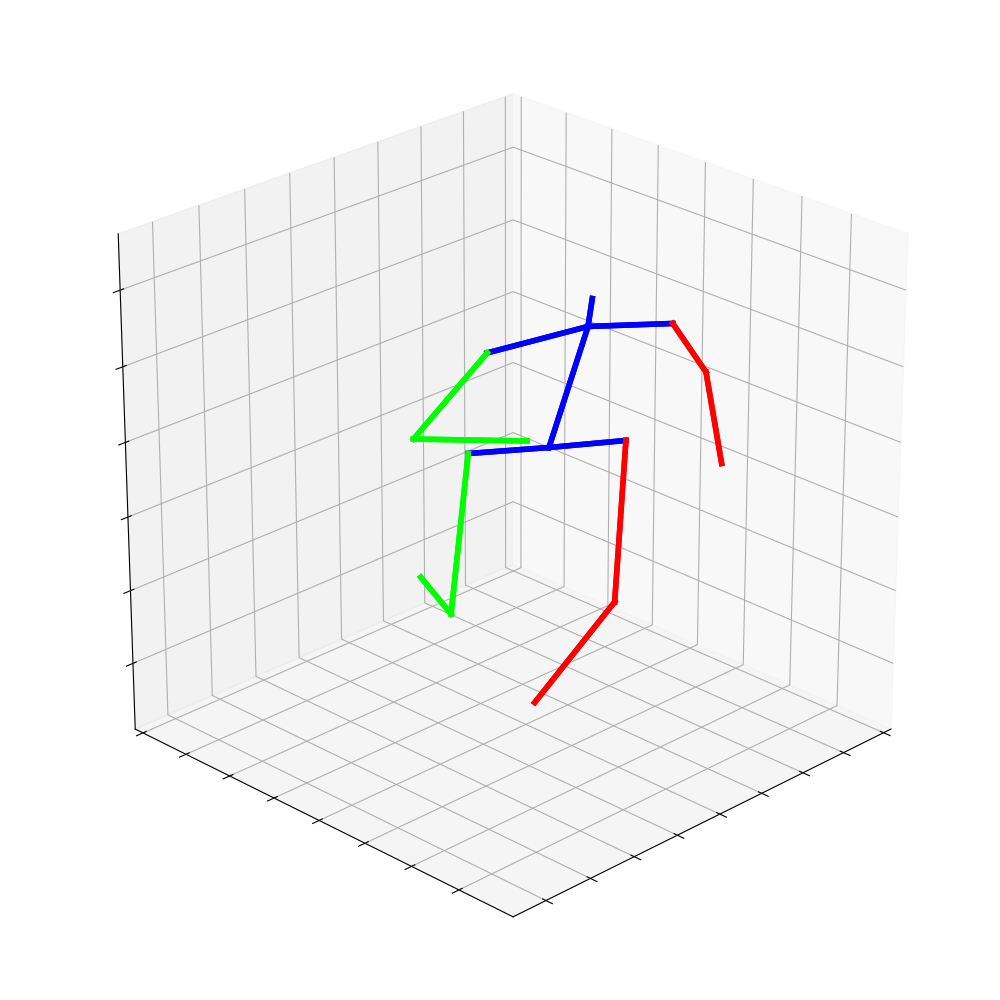
\includegraphics[width=.45\textwidth]{figures/qualitative_results/gt_1723.png}
			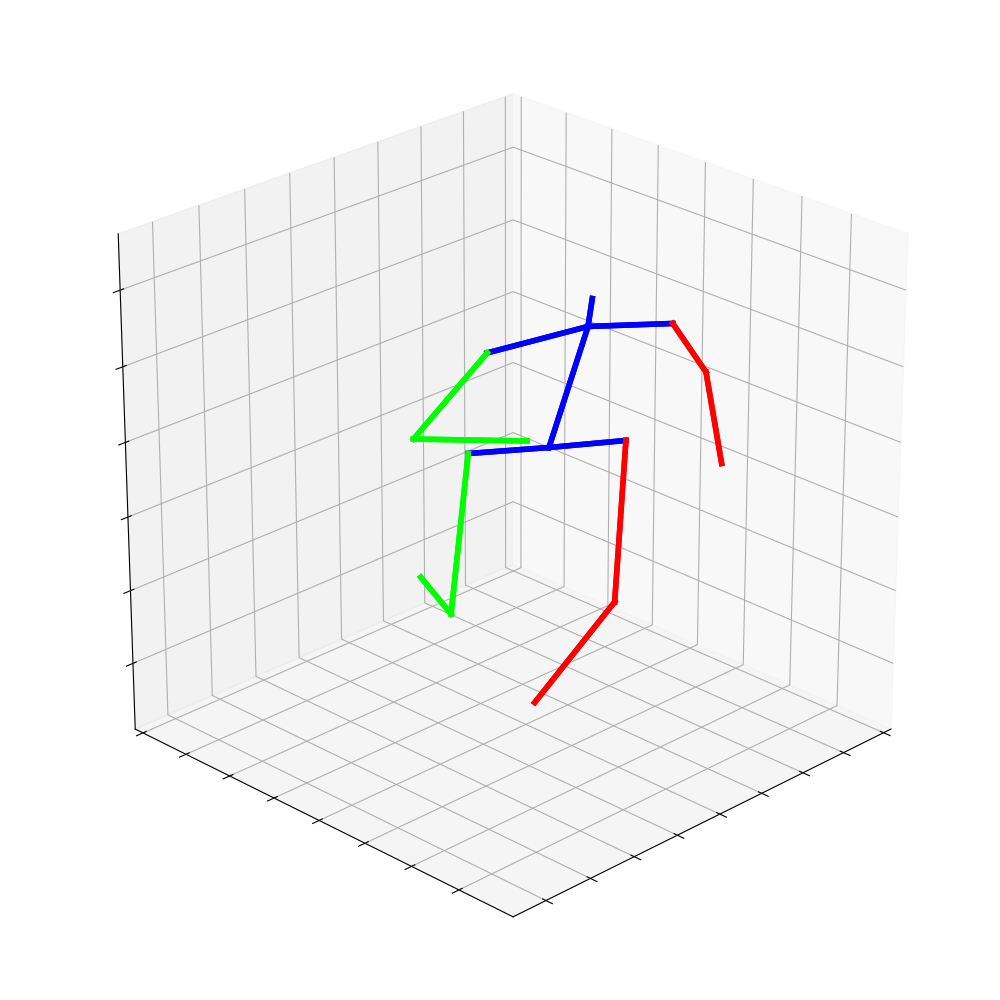
\includegraphics[width=.45\textwidth]{figures/qualitative_results/inferred_1723.png}
			}
		\end{minipage}
		\hspace{2mm}
		\begin{minipage}{.35\textwidth}
			\centering{
			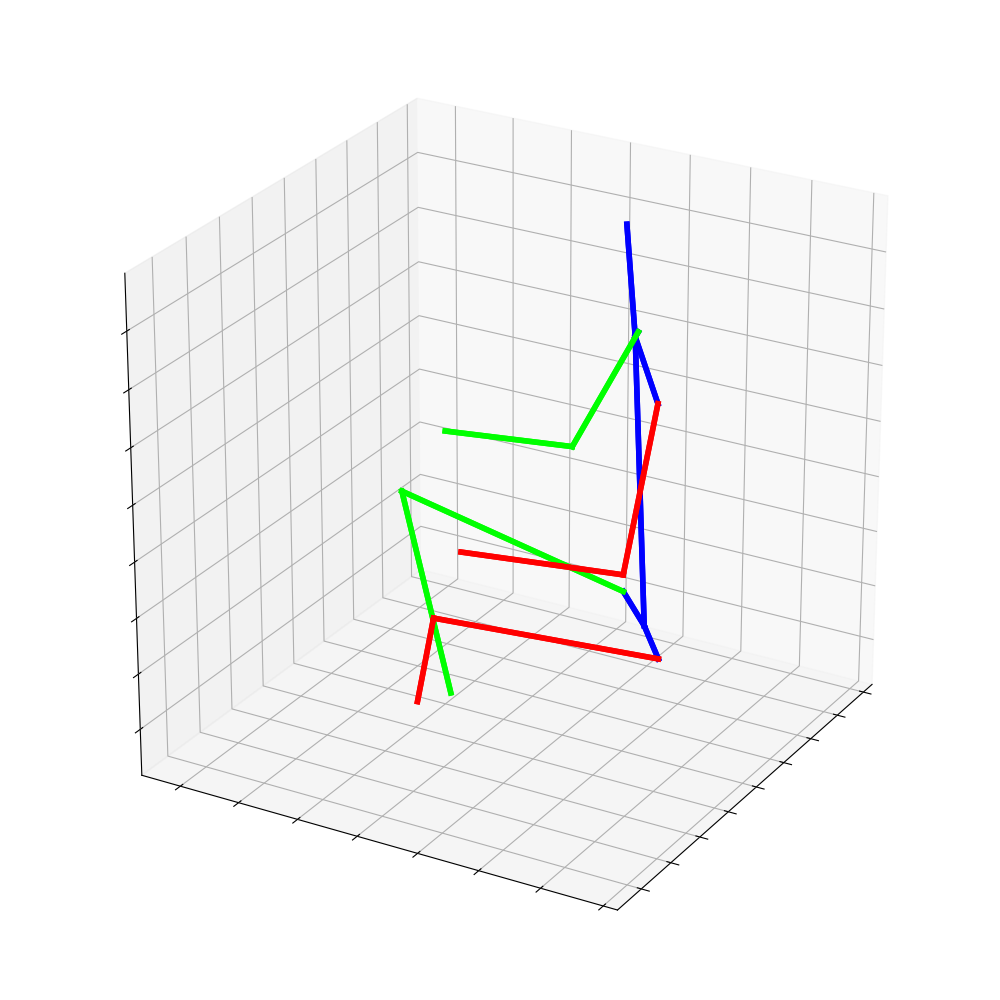
\includegraphics[width=.45\textwidth]{figures/qualitative_results/gt_3361.png}
			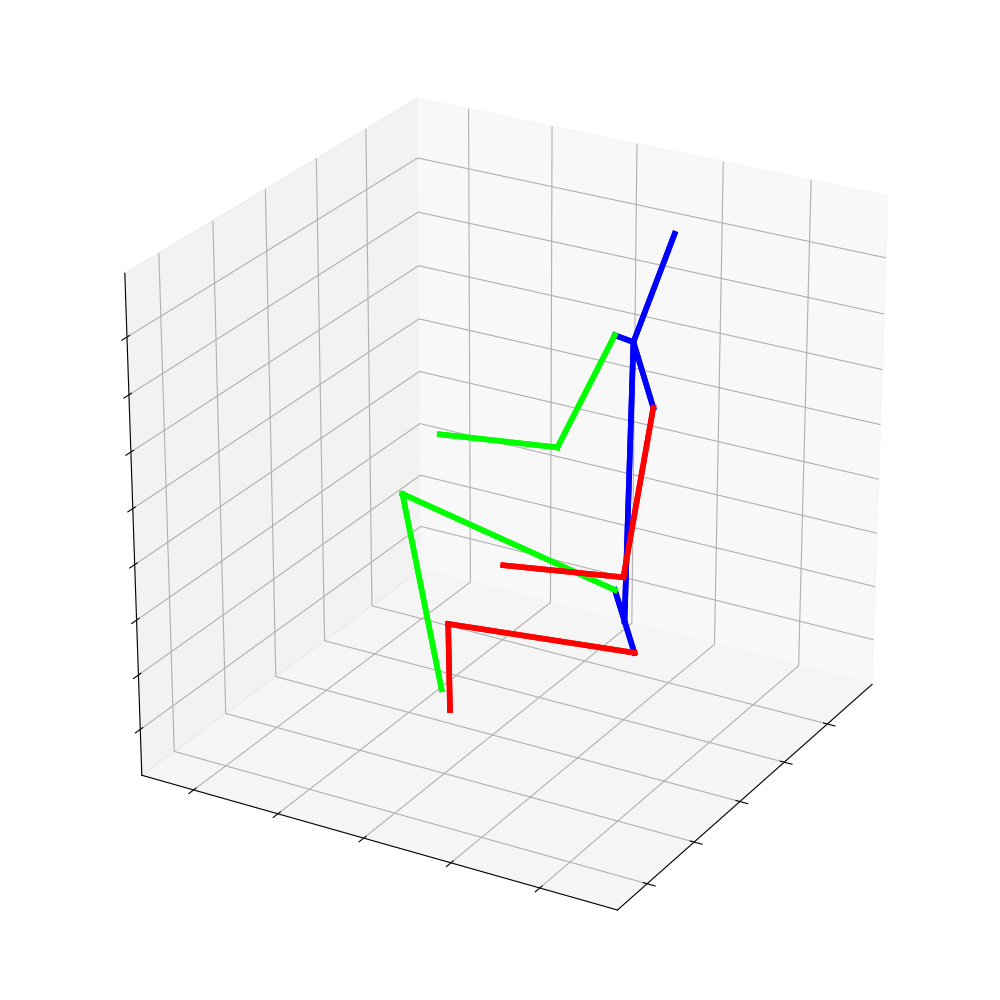
\includegraphics[width=.45\textwidth]{figures/qualitative_results/inferred_3361.png}
			}
		\end{minipage}
		\hspace{2mm}
		\begin{minipage}{.35\textwidth}
			\centering{
			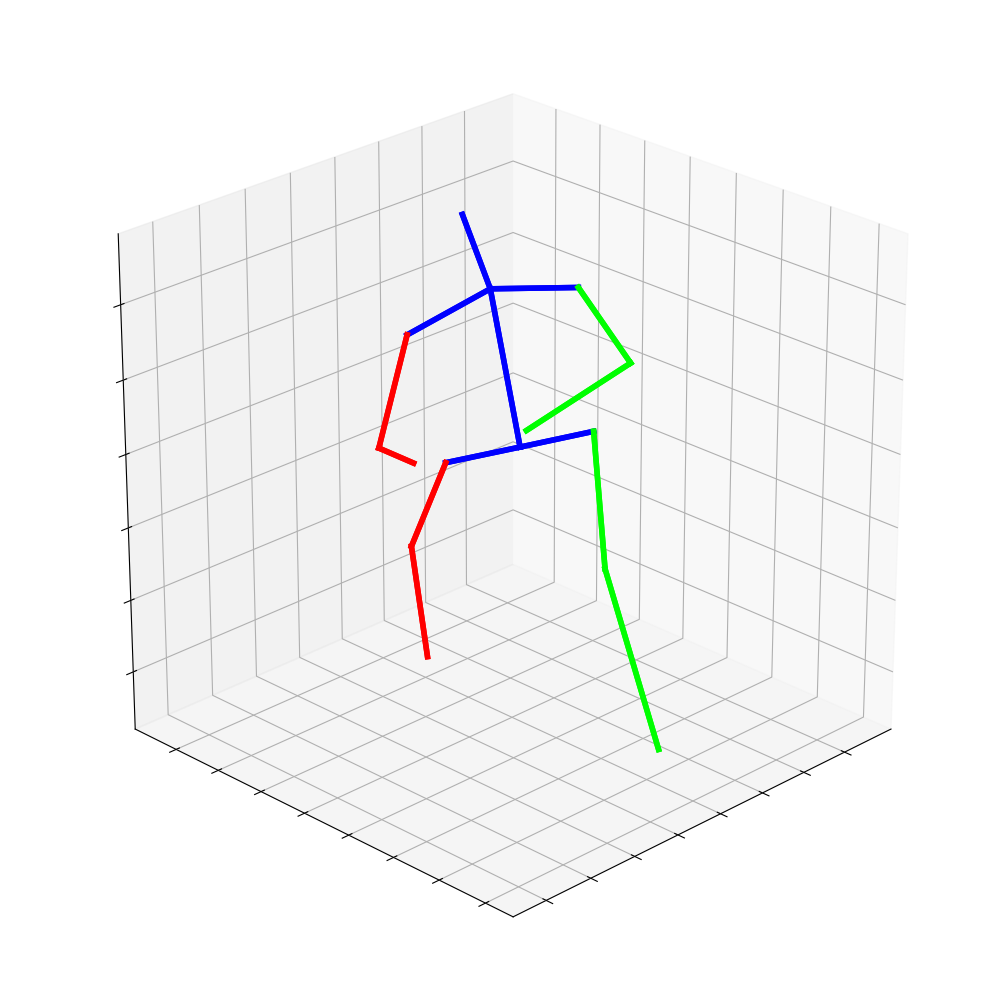
\includegraphics[width=.45\textwidth]{figures/qualitative_results/gt_4301.png}
			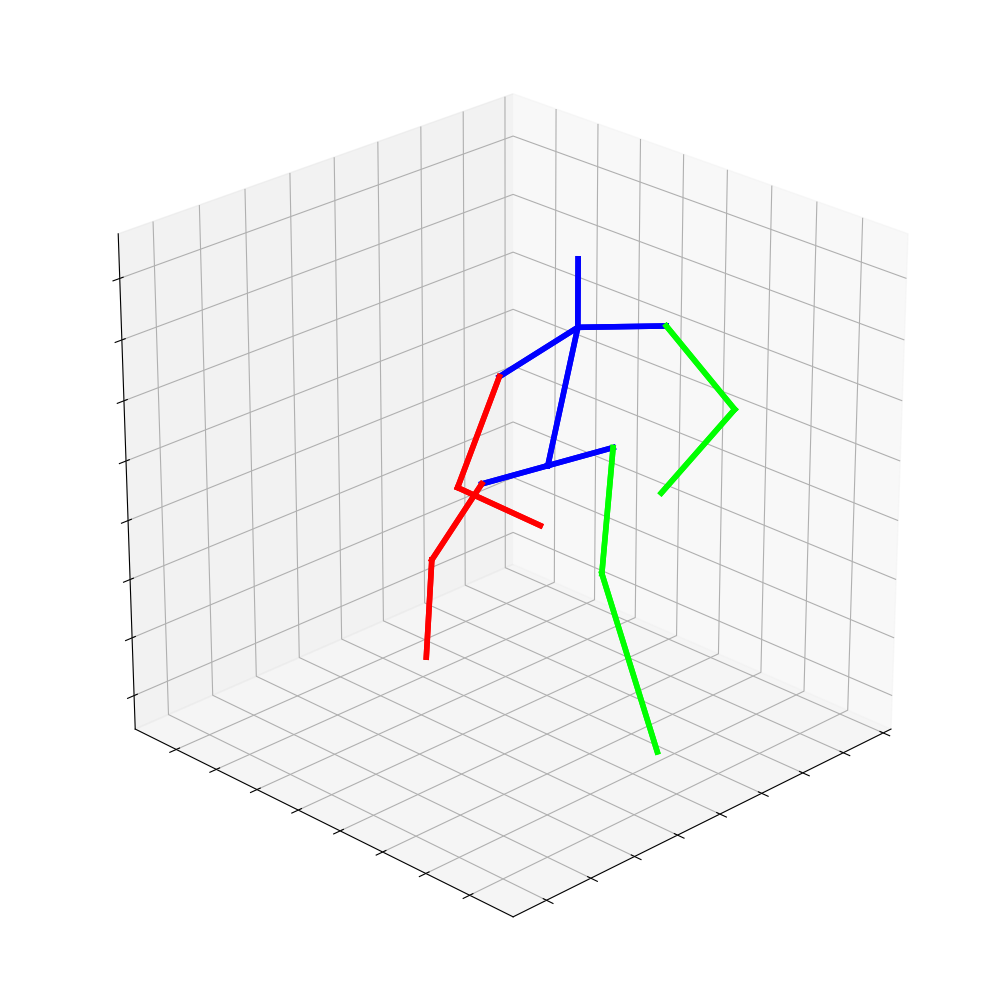
\includegraphics[width=.45\textwidth]{figures/qualitative_results/inferred_4301.png}
			}
		\end{minipage}
	}
	\makebox[\textwidth][c]{
		\begin{minipage}{.35\textwidth}
			\centering{
				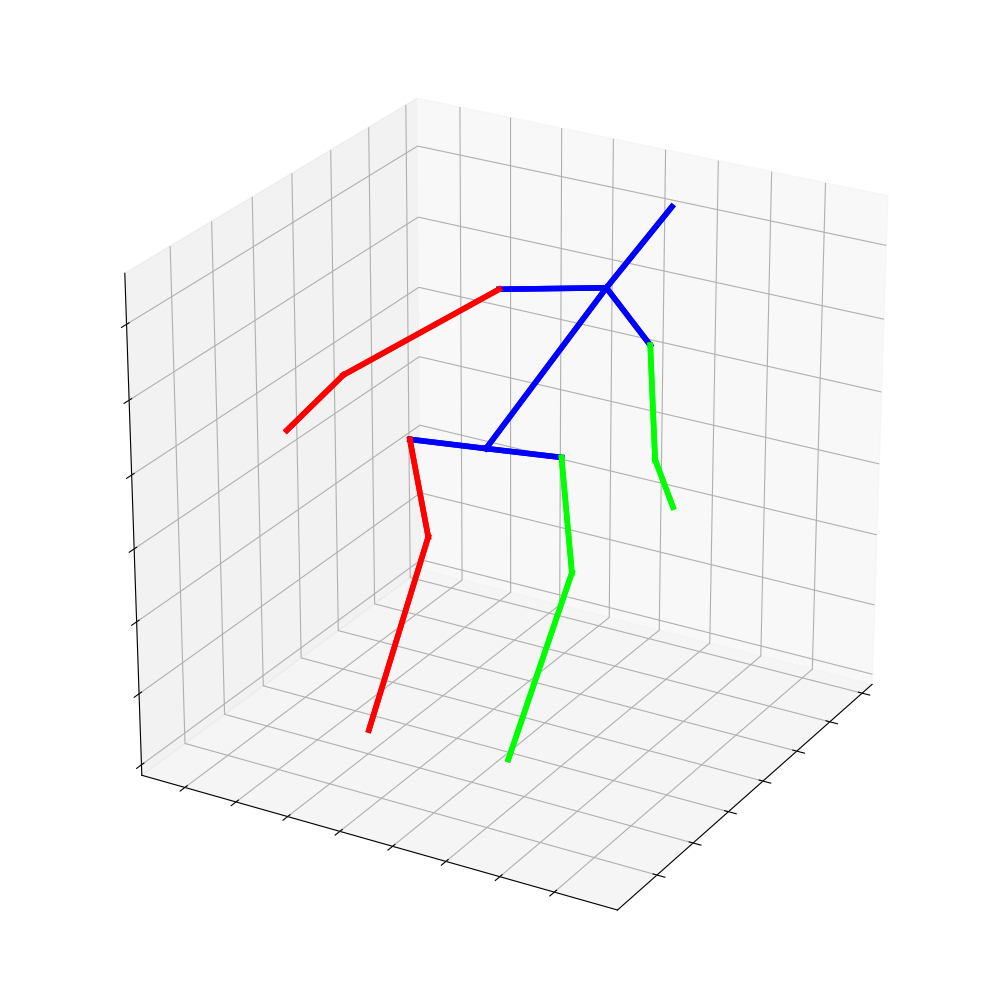
\includegraphics[width=.45\textwidth]{figures/qualitative_results/gt_original_2212.png}
				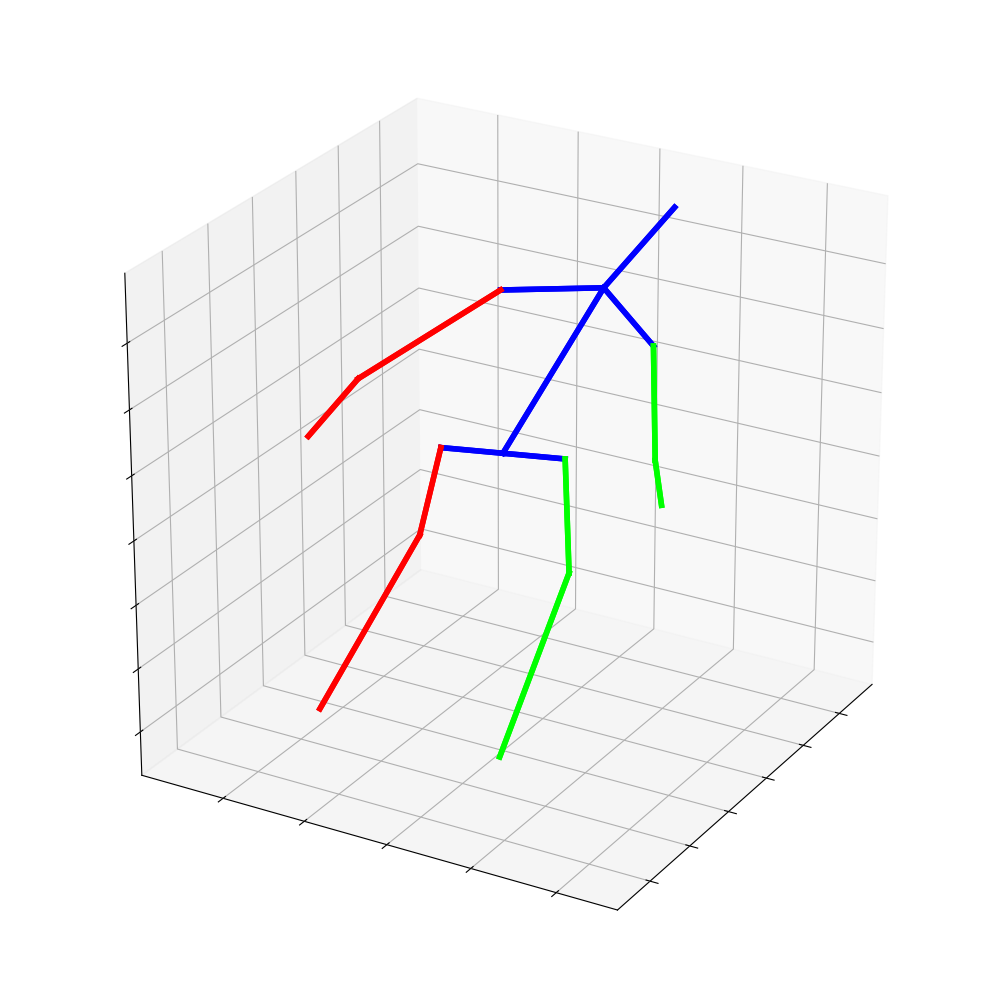
\includegraphics[width=.45\textwidth]{figures/qualitative_results/inferred_original_2212.png}
			}
		\end{minipage}
		\hspace{2mm}
		\begin{minipage}{.35\textwidth}
			\centering{
				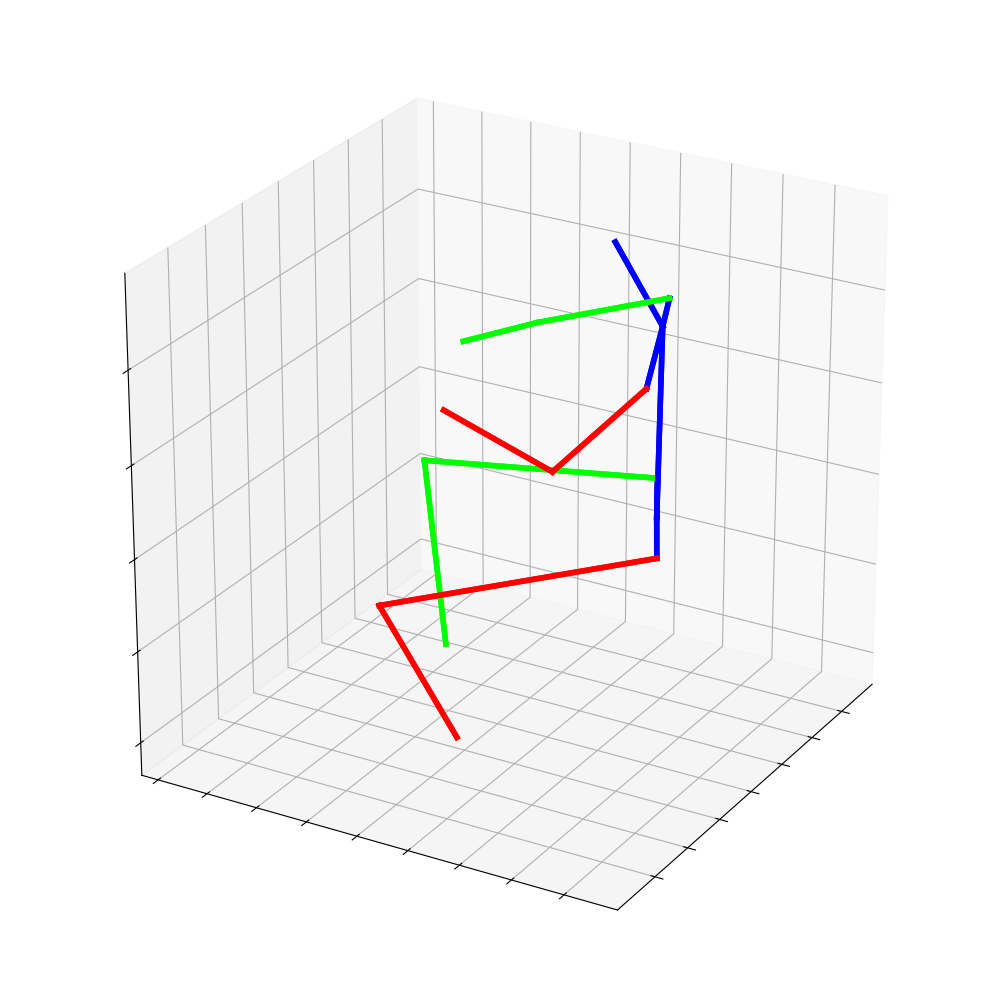
\includegraphics[width=.45\textwidth]{figures/qualitative_results/gt_original_2546.png}
				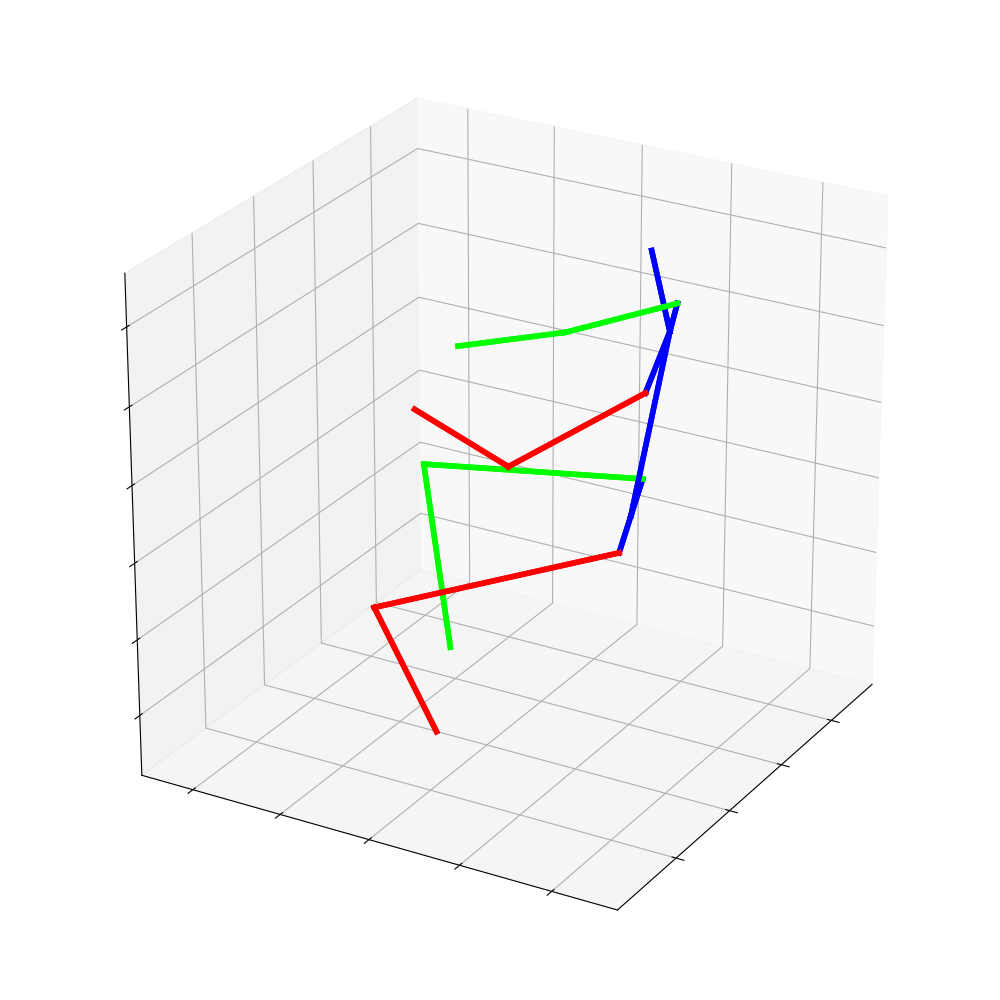
\includegraphics[width=.45\textwidth]{figures/qualitative_results/inferred_original_2546.png}
			}
		\end{minipage}
		\hspace{2mm}
		\begin{minipage}{.35\textwidth}
			\centering{
				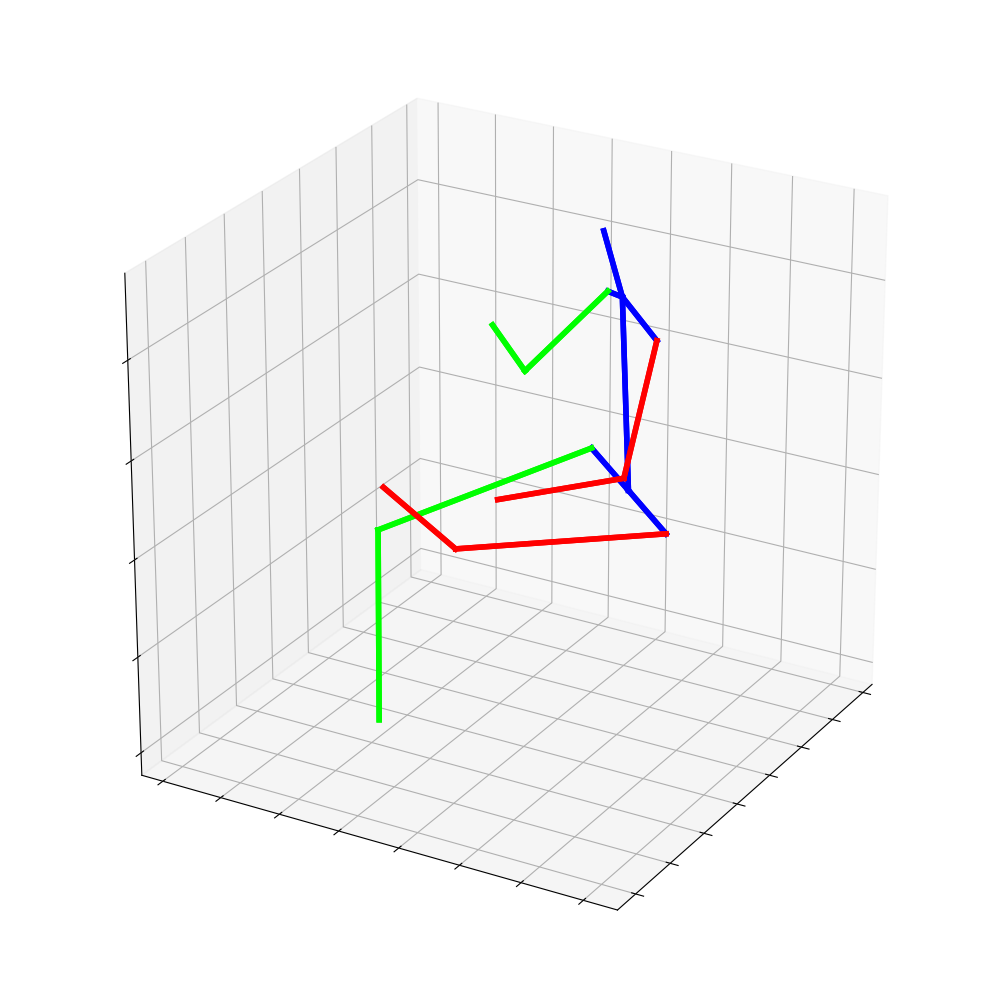
\includegraphics[width=.45\textwidth]{figures/qualitative_results/gt_original_3529.png}
				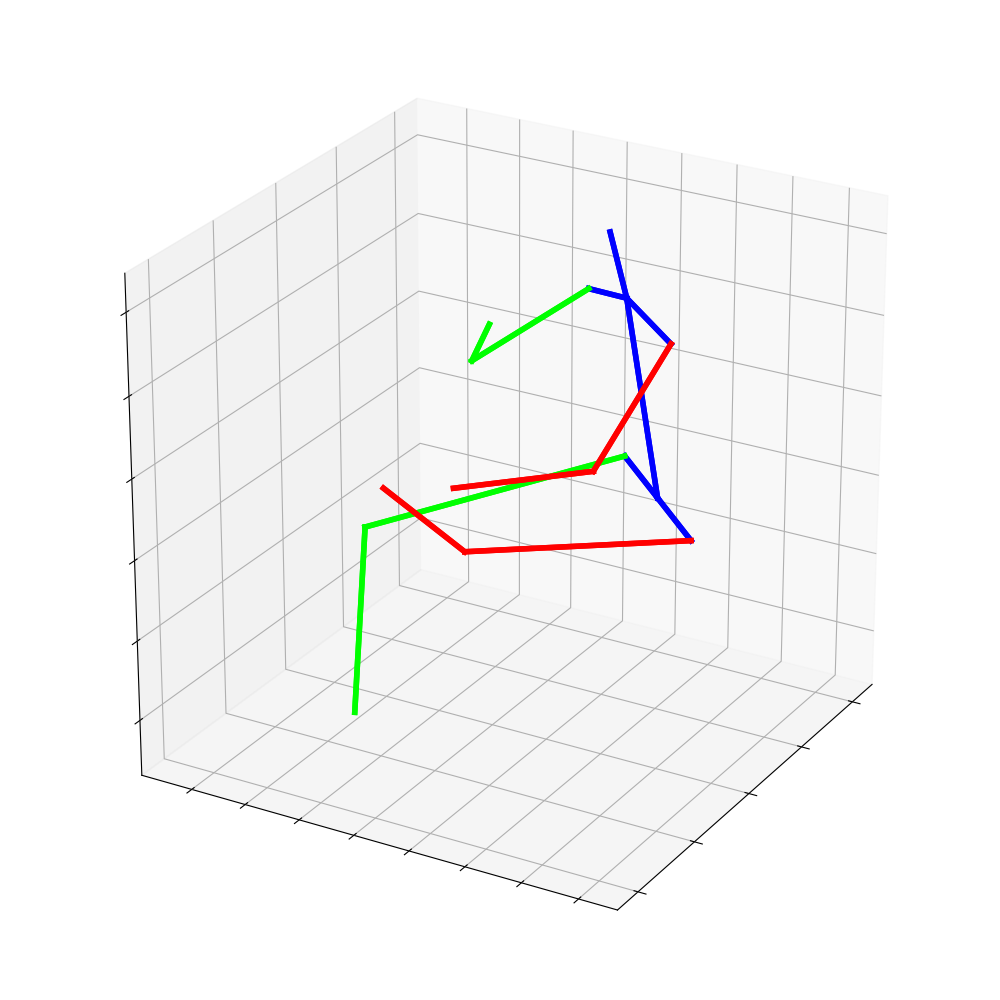
\includegraphics[width=.45\textwidth]{figures/qualitative_results/inferred_original_3529.png}
			}
		\end{minipage}
	}
	\caption{
	Qualitative results for the rebuilt system trained with synthetic poses.
	The first row shows poses inferred from synthetic 2D poses, the second poses inferred from the 2D poses included in Human3.6M.
	Ground truth poses are left and inferred poses right for each pair of poses.
	All poses were selected randomly.
	}
	\label{fig:qualitative-results}
	\info[inline]{All figures obtained with best.ckpt-16161 from e\_03\_07\_original.json}
\end{figure}

\autoref{fig:qualitative-results} shows some qualitative results for synthetic 2D poses (first row) and 2D poses from Human3.6M (second row).
All of the randomly selected inferred poses closely resemble the ground truth poses.
Usual failures are limbs that are bent in a slightly different direction than in the ground truth pose (e.g. the head in the top center example and the upper body in top right example).
Overall, all of the 3D poses could be successfully recovered from the 2D poses, with some showing minor differences compared to the ground truth poses.

The system is also evaluated for a different dataset.
On the test data of TotalCapture \cite{trumble17}, the average MPJPE is 68.3mm and and 100.2mm for Protocol 1 and 2, respectively (\autoref{tbl:results-original-totalcapture}).
The pose structure in this dataset is slightly different from Human3.6M, which could explain the higher error.
The most noticeable difference is the angle between the two hips.
In Human3.6M, this angle measures 180 degrees and the spine is perpendicular to the hips, whereas in TotalCapture the angle is substantially smaller (see \autoref{fig:human-totalcapture}).
Also, the spine appears to be shorter and the head longer for the poses from Human3.6M.
Although the results for TotalCapture are slightly worse, they still show that the system generalizes to unseen data in a reasonable way.

\begin{figure}
	\centering
	\begin{minipage}{.45\textwidth}
		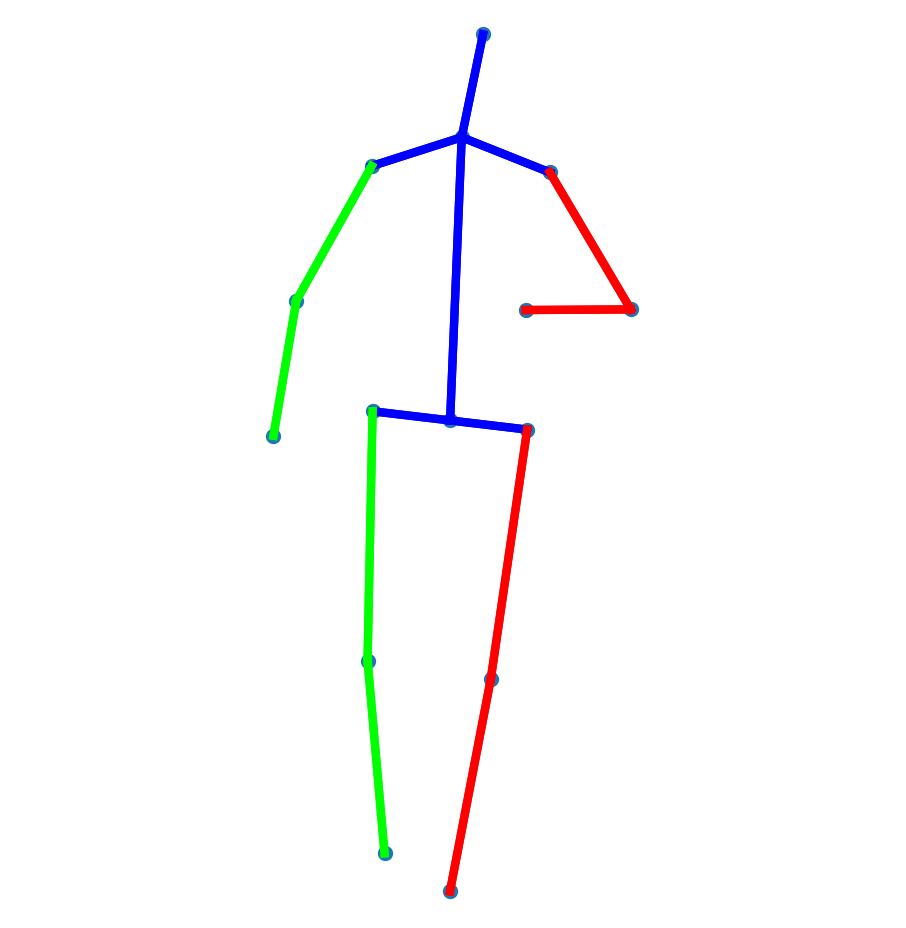
\includegraphics[width=.45\textwidth]{figures/2D_pose_human36m_1701.png}
		\scalebox{-1}[1]{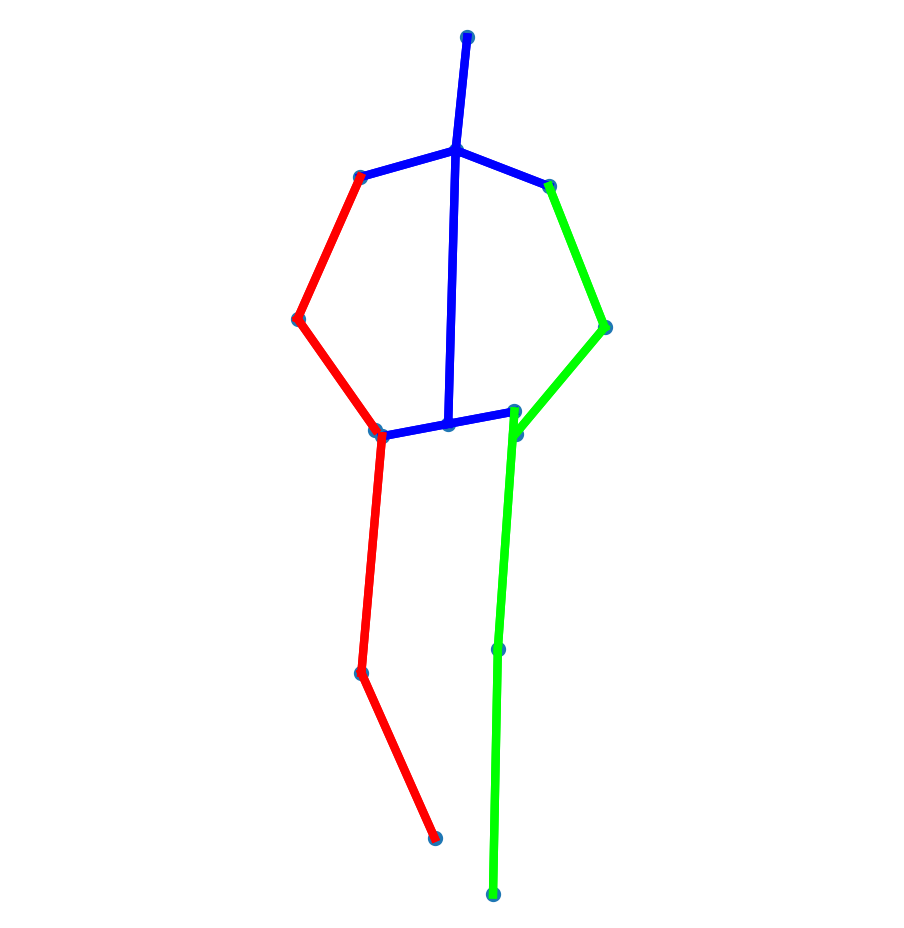
\includegraphics[width=.45\textwidth]{figures/2D_pose_human36m_4280.png}}
	\end{minipage}
	\hspace{5mm}
	\begin{minipage}{.45\textwidth}
	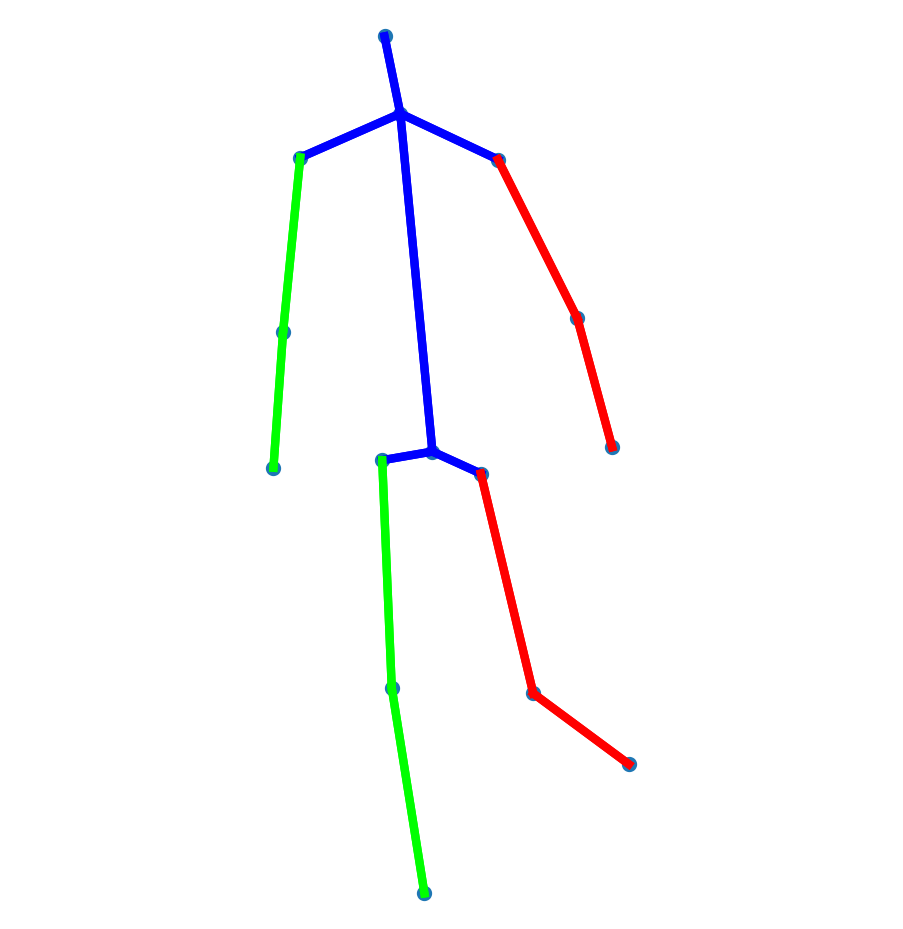
\includegraphics[width=.45\textwidth]{figures/2D_pose_totalcapture_24437.png}
	\scalebox{-1}[1]{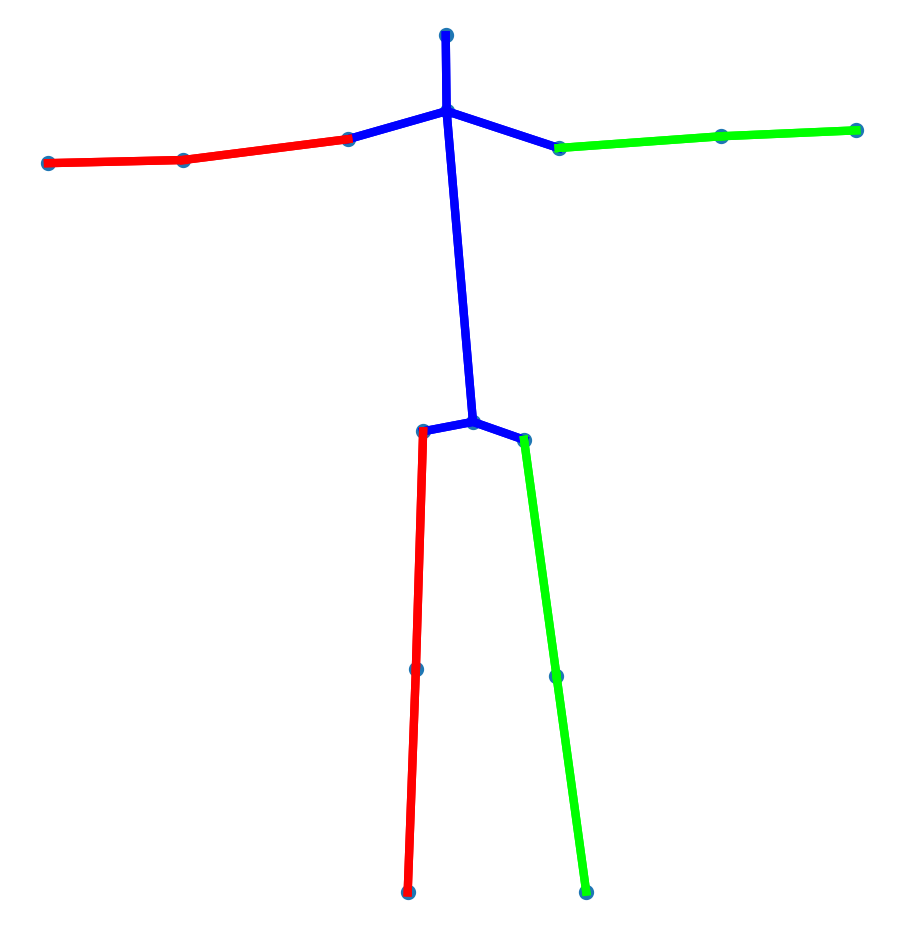
\includegraphics[width=.45\textwidth]{figures/2D_pose_totalcapture_102156.png}}
	\end{minipage}
	\caption{Comparison of two poses from the Human3.6M dataset (left) and two poses from the TotalCapture dataset (right).}
	\label{fig:human-totalcapture}
\end{figure}


\subsection{Results for Training with Augmented and Real Data}
\label{sec:results-augmented}
The results for the test data of the Human3.6M dataset are not quite satisfying, as they are only useful when rotation plays no role.
The reasons for the worse results may have different origins:
A simple explanation is that machine learning systems tend to perform better on data which is more similar to the training data.
For the synthetic testing data this is certainly the case.
However, the results for Protocol 1 show that the poses are already sensible and only seem to lack the right orientation.
Another reason might be that Human3.6M's monocular 2D poses are in fact being normalized, both in scale and position, other than the synthetic data, which is already naturally normalized in position (and also almost in scale).

In order to figure out whether the first conjecture contributes to the discrepancy, the monocular 2D poses are added to the training set.
A lower MPJPE would indicate that it does.
For training, the generator receives both real and synthetic poses at a 1:1 ratio.
As described in \autoref{sec:network}, during training the generator tries to learn the real data distribution.
In order to have a chance to achieve this, it must be able to generate poses similar to the real poses. 
This comes down to the Random Projection Layer, where the poses are projected to 2D with the root joint lying on the principal axis of the camera at a distance of $10$.
2D poses projected with a camera distance other than $10$ or with a camera that is not centered at the root joint are inherently different.
This will further be elaborated on in \autoref{sec:effects-of-normalization}.
Thus there are two options:
Projecting the generated 3D poses with a camera distance and offset similar to the real data or feeding only data to the discriminator that resembles the generator's output.
As the real camera distance might not be known in general, and offsets would still need to be sampled, the second option is chosen.
This means the discriminator still only receives synthetic poses for training.

\begin{table}[]	
	\centering
	\begin{tabularx}{\textwidth}{l *{8}{Y}}
		\toprule
		Method & Direct. & Discuss & Eat & Greet & Phone & Pose & Purchase & Sit \\
		\midrule
		Synthetic & 48.8 & 51.5 & 41.5 & 57.7 & 49.4 & 54.3 & 48.8 & 50.0 \\
		Human3.6M & 48.8 & 51.5 & 41.5 & 57.7 & 49.4 & 54.3 & 48.8 & 50.0 \\
		\bottomrule
		\toprule
		Method & SitDown & Smoke & TPhoto & Wait & Walk & WDog & WTog. & \textbf{Avg.}\\
		\midrule
		Synthetic & 64.3 & 51.9 & 64.6 & 57.1 & 54.3 & 57.9 & 53.2 & \textbf{54.8} \\
		Human3.6M & 48.8 & 51.5 & 41.5 & 57.7 & 49.4 & 54.3 & 48.8 & 50.0 \\
		\bottomrule
	\end{tabularx}
	\caption{
		Comparison of the MPJPEs of the replicated system trained with monocular 2D poses from the Human3.6M dataset and synthetic data at a 1:1 ratio.
		The results are given for synthetic data and 2D poses from the Human3.6M dataset \cite{ionescu14}.
		The results were obtained using \textbf{Protocol 2}. The MPJPEs are given in millimeters.
	 }
	\label{tbl:results-real-and-synthetic-protocol2}
	\info[inline]{}
\end{table}

\autoref{tbl:results-real-and-synthetic-protocol2} shows the results for both synthetic data and the monocular 2D test poses from Human3.6M for this data configuration.
While the results for the synthetic data are approximately the same as the ones in the previous section, the results for the Human3.6M poses improved by almost $8$mm to $72.5$mm.

In \cite{drover18}, the authors report training the system with augmented poses obtained from projecting the 3D poses with cameras that are similar to the four real cameras available in the Human3.6M dataset.
Compared to the above approach of synthetically generating 2D poses, here, the cameras are fixed and have similar extrinsic parameters as the real ones.
A training with this setup showed no major improvement to the previous number.
For training, the positions of eight additional cameras were chosen to have equidistant azimuth angles and a camera distance between $4.6$m and $5.4$m, which comes close to the four real cameras.
The Protocol 2 MPJPE for this setup is at $71.8$mm.

These results have both positive and negative ramifications:
On the one hand, when the system is trained with real world data from a specific application, it will perform better in that application, compared to a pre-trained model.
On the other hand, this shows that the system is not able to generalize to all kinds of human poses with the same quality. 
